\documentclass[11pt,a4paper]{article}
\usepackage[margin=1in]{geometry}
\usepackage{microtype}
\usepackage{hyperref}
\usepackage{enumitem}
\usepackage{graphicx}
\usepackage{xcolor}
\usepackage{booktabs}
\usepackage{tabularx}
\usepackage{array}
\usepackage{caption}
\usepackage{float}
\usepackage{tikz}
\usetikzlibrary{arrows.meta,positioning,fit,backgrounds,calc}
\usepackage{pgfplots}
\pgfplotsset{compat=1.18}

\hypersetup{colorlinks=true, linkcolor=black, urlcolor=accent,
  citecolor=black}
\captionsetup{font=small, labelfont=bf, skip=6pt}
\setlist{leftmargin=0.7cm, itemsep=2pt, topsep=4pt}

% -----------------------------------------------------
% bvraghav-tiet-ucs503p-article.sty
% -----------------------------------------------------

% Variable: Lab Instructor
\makeatletter \newcommand{\BvrSetLabInstructor}[1]{%
  \gdef\Bvr@LabInstructor{#1}}
% default
\newcommand{\Bvr@LabInstructor}{Dr. Paramveer Kaur}
% public accessor
\newcommand{\BvrLabInstructorValue}{\Bvr@LabInstructor}
\makeatother

% Add subtitle
\usepackage{titling}
% -- Set title bold
\pretitle{\begin{center}\bfseries\fontsize{18bp}{18bp}\selectfont}
\makeatletter
\newcommand{\BvrSubtitle}[1]{%
  \posttitle{%
    \par\end{center}
    \begin{center}\large#1\end{center}
    \vskip 0.5em}%
}
\makeatother

% Hints in the section title(s)
\newcommand{\BvrHint}[1]{%
  {\normalfont\normalsize\itshape\hfill #1}}

% -----------------------------------------------------
% Colours. Each one means one thing, everywhere in the
% report: ink is the observation, accent is Pawan,
% muted is a baseline.
\definecolor{ink}{HTML}{1F2933}
\definecolor{accent}{HTML}{0B6E99}
\definecolor{muted}{HTML}{8A939B}
\definecolor{warn}{HTML}{C2410C}
\definecolor{rule}{HTML}{CBD2D9}

\newcommand{\ugm}{$\mu$g/m$^3$}
\newcommand{\pmtf}{PM$_{2.5}$}
\newcommand{\done}{\textcolor{accent}{\textbf{done}}}
\newcommand{\changed}{\textcolor{warn}{\textbf{changed}}}
\newcommand{\partly}{\textcolor{warn}{\textbf{partly}}}
\newcommand{\notyet}{\textcolor{muted}{\textbf{not yet}}}

% Every figure quoted below. Generated from data/ by
% scripts/report_figures.py; do not edit by hand.
% Generated by scripts/report_figures.py. Do not edit.
\newcommand{\NAll}{488}
\newcommand{\ModelAll}{8.63}
\newcommand{\TextAll}{7.66}
\newcommand{\OperAll}{12.36}
\newcommand{\CamsAll}{41.87}
\newcommand{\SkillOpAll}{30.1}
\newcommand{\SkillTxAll}{-12.7}
\newcommand{\LossTxAll}{12.7}
\newcommand{\NCalm}{425}
\newcommand{\ModelCalm}{8.11}
\newcommand{\TextCalm}{7.12}
\newcommand{\OperCalm}{11.35}
\newcommand{\CamsCalm}{43.89}
\newcommand{\SkillOpCalm}{28.5}
\newcommand{\SkillTxCalm}{-13.8}
\newcommand{\LossTxCalm}{13.8}
\newcommand{\NBurn}{63}
\newcommand{\ModelBurn}{12.16}
\newcommand{\TextBurn}{11.32}
\newcommand{\OperBurn}{19.14}
\newcommand{\CamsBurn}{28.21}
\newcommand{\SkillOpBurn}{36.5}
\newcommand{\SkillTxBurn}{-7.4}
\newcommand{\LossTxBurn}{7.4}
\newcommand{\NLive}{47}
\newcommand{\ModelLive}{4.33}
\newcommand{\TextLive}{4.17}
\newcommand{\OperLive}{7.50}
\newcommand{\CamsLive}{41.17}
\newcommand{\SkillOpLive}{42.3}
\newcommand{\SkillTxLive}{-3.9}
\newcommand{\LossTxLive}{3.9}
\newcommand{\BacktestFirst}{4 April 2025}
\newcommand{\BacktestLast}{7 October 2026}
\newcommand{\PoorDays}{9}
\newcommand{\PoorCaught}{0}
\newcommand{\PoorFlagged}{0}
\newcommand{\ModDays}{63}
\newcommand{\ModCaught}{17}
\newcommand{\ModFlagged}{25}
\newcommand{\ModOperCaught}{35}
\newcommand{\ModOperFlagged}{67}
\newcommand{\MaxForecast}{75}
\newcommand{\PeakDay}{2 November 2025}
\newcommand{\PeakObs}{141}
\newcommand{\PeakModel}{63}
\newcommand{\TopFiveRatio}{44}
\newcommand{\LiveFirst}{7 September}
\newcommand{\LiveLast}{11 October}
\newcommand{\LiveExpected}{35}
\newcommand{\LiveIssued}{24}
\newcommand{\LiveScored}{18}
\newcommand{\LiveMAE}{6.61}
\newcommand{\LiveBand}{13}
\newcommand{\LiveInside}{10}
\newcommand{\Rows}{589}
\newcommand{\RowsFirst}{19 February 2025}
\newcommand{\RowsObserved}{585}
\newcommand{\RowsThin}{48}
\newcommand{\RowsLive}{57}
\newcommand{\RowsSpan}{600}
\newcommand{\Usable}{528}
\newcommand{\RatioLow}{1.2}
\newcommand{\RatioHigh}{3.9}


% -----------------------------------------------------

\title{Pawan: Locally Calibrated Next-Day Air Quality
  Forecasting for Patiala}

\BvrSetLabInstructor{Dr. Paramveer Kaur}

\BvrSubtitle{%
  Prototype stage: a forecast issued every morning, and
  an honest account of how good it is
  \\[0.4em]
  Progress Report for UCS503P \\
  Submitted to: \BvrLabInstructorValue \\ \bfseries
  Thapar Institute of Engineering and Technology%
}

\author{
  Gurkirpa Singh, CSED%
  \thanks{Roll No: \texttt{1024170378}, %
    Email: \texttt{gsarao\_be24\@thapar.edu}}
  \and
  Ketubh Bansal, CSED%
  \thanks{Roll No: \texttt{1024170399}, %
    Email: \texttt{kketubh1\_be24\@thapar.edu}}
  \and
  Aayush Kandhol, CSED%
  \thanks{Roll No: \texttt{1024170379}, %
    Email: \texttt{akandhol\_be24\@thapar.edu}}
}

\date{12 October 2026}

\begin{document}
\maketitle

\begin{center}
\fcolorbox{rule}{white}{\begin{minipage}{0.92\linewidth}
\vspace{0.5em}
\textbf{At a glance.} Pawan has issued a next-day \pmtf{} forecast
for the Model Town station every morning since \LiveFirst, without
anyone running it. It is checked against what the station later
measures, and the record is public at
\href{https://blakkbird.github.io/ucs503p-202627odd-Project-P1.v1/forecast/}{the
project page}.

\smallskip
Over a walk-forward backtest of \NAll{} days it beats the honest
baseline, persistence from the freshest reading available at issue
time, by \textbf{\SkillOpCalm\%} in the calm season and
\textbf{\SkillOpBurn\%} in the burning season. The proposal's
targets were 10\% and 20\%. It does not beat persistence from
\emph{yesterday's} reading, which nobody has at issue time, and it
does not see pollution spikes coming: it flagged none of the
\PoorDays{} days that reached the \emph{Poor} band. Both are
reported below rather than left out, and the second sets the
direction for the next iteration.
\vspace{0.3em}
\end{minipage}}
\end{center}

\section{Where the project stands%
  \BvrHint{\ldots the short version}}

The proposal promised three things: a pipeline that runs on its
own, an evaluation that cannot flatter itself, and a correction
that beats persistence by a stated margin. All three exist.

\begin{itemize}
  \item \textbf{The pipeline runs unattended.} A scheduled job
    collects the station's observations, the CAMS global forecast,
    forecast weather and satellite fire detections every morning,
    refits the model, issues tomorrow's forecast, rebuilds the
    project page and commits all of it to the repository. The
    table now holds \Rows{} days, from \RowsFirst{} onwards.
  \item \textbf{The evaluation is walk-forward and leakage-checked.}
    Every scored forecast comes from a model fitted only on days
    before it, using only what had been published by 09:00 the
    day before. Forecasts, once issued, are frozen.
  \item \textbf{Both accuracy targets are met} against operational
    persistence, on \NCalm{} calm-season days and \NBurn{}
    burning-season days, including the whole of the 2025 season.
\end{itemize}

What is not yet good enough is equally definite. The model is a
good forecaster of an ordinary day and a poor forecaster of a bad
one: its largest prediction across the whole backtest is
\MaxForecast{}~\ugm, and the worst day on record reached
\PeakObs{}. Section~\ref{sec:eval} sets out the numbers and
Section~\ref{sec:plan} the plan.

\section{Proposal against prototype%
  \BvrHint{\ldots what changed and why}}

\begin{table}[H]
\centering
\small
\begin{tabularx}{\linewidth}{>{\raggedright\arraybackslash}p{4.6cm}
  l >{\raggedright\arraybackslash}X}
\toprule
\textbf{Proposed} & \textbf{Status} & \textbf{Note} \\
\midrule
Ingestion adapters for observations, forecast and fires
  & \done & One adapter per source, each validating response
    content rather than status codes. \\
Scheduled daily record carrying forecast issue time
  & \done & 08:00 IST via GitHub Actions; \RowsLive{} rows carry
    a recorded issue date. \\
Baselines over a fixed period
  & \done & Persistence twice, climatology, raw CAMS. See
    Section~\ref{sec:baselines}. \\
A correction that beats persistence
  & \done & Against operational persistence; not against textbook
    persistence. \\
Gradient boosted trees, linear model alongside
  & \changed & Ridge regression only, written by hand. Reasons in
    Section~\ref{sec:method}. \\
Continuous integration on every change
  & \done & Lint and \texttt{pytest} (100 tests) gate every pull
    request and every data commit. \\
Published dashboard
  & \done & Forecast and results pages, regenerated from the data
    on every run. \\
Fire activity and wind features
  & \done & Lagged fire counts and wind components, in the model
    since week 5. \\
Band classification and advisory rule
  & \partly & Bands shown and scored. The advisory is measured and
    fails; Section~\ref{sec:fails}. \\
Rolling-origin backtest over a full season
  & \done & \NAll{} days, \BacktestFirst{} to \BacktestLast. \\
Scheduled retraining
  & \done & The model is refitted from scratch every morning. \\
Feature importance
  & \done & Standardised weights published on the results page. \\
\bottomrule
\end{tabularx}
\caption{Items from the proposal's scope, as they stand.}
\end{table}

\section{The system as built%
  \BvrHint{\ldots engineering focus}}

\subsection{Architecture}

Figure~\ref{fig:arch} is the whole system. There is no server and
no database. The repository is the system of record: the dataset is
a CSV file in git, every change to it is a commit, and the public
page is built from the same files the model reads.

\begin{figure}[H]
\centering
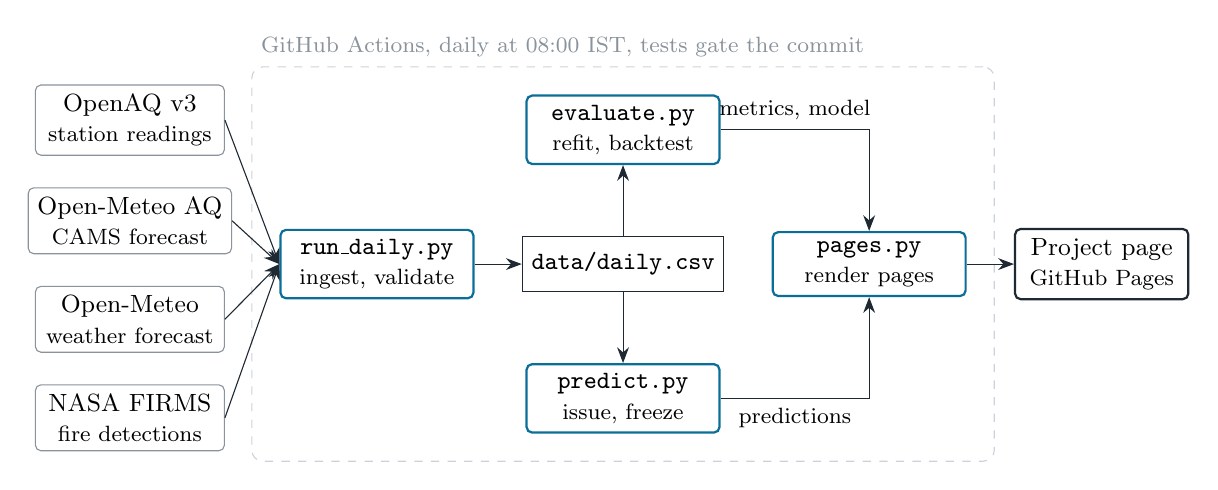
\begin{tikzpicture}[
  font=\small,
  node distance=4mm and 6mm,
  srcbox/.style={draw=muted, rounded corners=2pt, minimum width=2.4cm,
    minimum height=7mm, align=center, fill=white},
  stage/.style={draw=accent, thick, rounded corners=2pt,
    minimum width=2.45cm, minimum height=8mm, align=center,
    fill=white},
  filebox/.style={draw=ink, minimum width=2.45cm, minimum height=7mm,
    align=center, font=\small\ttfamily, fill=white},
  outbox/.style={draw=ink, thick, rounded corners=2pt,
    minimum width=2.2cm, minimum height=8mm, align=center,
    fill=white},
  flowline/.style={-{Stealth[length=2mm]}, draw=ink},
]
  % sources
  \node[srcbox] (oaq) {OpenAQ v3\\\footnotesize station readings};
  \node[srcbox, below=of oaq] (cams) {Open-Meteo AQ\\\footnotesize CAMS forecast};
  \node[srcbox, below=of cams] (wx) {Open-Meteo\\\footnotesize weather forecast};
  \node[srcbox, below=of wx] (firms) {NASA FIRMS\\\footnotesize fire detections};

  % pipeline
  \node[stage, right=of cams, yshift=-5.5mm] (ingest)
    {\texttt{run\_daily.py}\\\footnotesize ingest, validate};
  \node[filebox, right=of ingest] (csv) {data/daily.csv};
  \node[stage, above=9mm of csv] (eval)
    {\texttt{evaluate.py}\\\footnotesize refit, backtest};
  \node[stage, below=9mm of csv] (pred)
    {\texttt{predict.py}\\\footnotesize issue, freeze};
  \node[stage, right=of csv] (pages)
    {\texttt{pages.py}\\\footnotesize render pages};
  \node[outbox, right=of pages] (site)
    {Project page\\\footnotesize GitHub Pages};

  \foreach \s in {oaq,cams,wx,firms} \draw[flowline] (\s.east) -- (ingest.west);
  \draw[flowline] (ingest) -- (csv);
  \draw[flowline] (csv) -- (eval);
  \draw[flowline] (csv) -- (pred);
  \draw[flowline] (eval.east) -| node[pos=0.25, above, font=\footnotesize]
    {metrics, model} (pages.north);
  \draw[flowline] (pred.east) -| node[pos=0.25, below, font=\footnotesize]
    {predictions} (pages.south);
  \draw[flowline] (pages) -- (site);

  % CI boundary
  \begin{scope}[on background layer]
    \node[draw=rule, dashed, rounded corners=4pt, inner sep=3.5mm,
      fit=(ingest)(eval)(pred)(pages),
      label={[font=\footnotesize, text=muted, anchor=south west]
        north west:GitHub Actions, daily at 08:00 IST, tests gate the commit}]
      (ci) {};
  \end{scope}
\end{tikzpicture}
\caption{Data flow. Grey boxes are external services, blue boxes
are the pipeline stages, and the dashed boundary is what runs
unattended each morning. \texttt{predict.py} applies the model that
\texttt{evaluate.py} has just refitted and saved.}
\label{fig:arch}
\end{figure}

\subsection{Components}

\begin{table}[H]
\centering
\small
\begin{tabularx}{\linewidth}{>{\ttfamily}l >{\raggedright\arraybackslash}X}
\toprule
\normalfont\textbf{Module} & \textbf{Responsibility} \\
\midrule
config.py & Every setting in one place: station, sensor ids, lags,
  validity rules, paths. \\
ingest/run\_daily.py & Fetches a rolling 30-day window of
  observations and tomorrow's forecast; fails the run if the
  observation feed has gone stale. \\
features.py & Turns the table into model rows, and is where the
  information-set rules live. \\
model.py & Ridge regression on standardised features, solved by
  hand; about eighty lines, standard library only. \\
evaluate.py & Walk-forward backtest, all baselines, the per-season
  and live-only splits; writes \texttt{metrics.json} and
  \texttt{model.json}. \\
predict.py & Issues tomorrow's forecast once, never rewrites it,
  attaches the outcome when it publishes. \\
pages.py & Renders the forecast and results pages from the JSON
  files. Nothing on the site is typed by hand. \\
scripts/ & One-off tools: history extension, archive backfill,
  model comparison, the figures in this report. \\
\bottomrule
\end{tabularx}
\caption{\texttt{code/} is 2{,}157 lines; \texttt{code/tests/} is a
further 1{,}153.}
\end{table}

\subsection{Rules the pipeline keeps}

\begin{itemize}
  \item \textbf{Standard library only at run time.} The ingest and
    the model import nothing outside Python. \texttt{requirements.txt}
    holds \texttt{pytest} and \texttt{ruff} and nothing else, so
    the daily job cannot break on a dependency upgrade.
  \item \textbf{A forecast is written once.} \texttt{predict.py}
    never rewrites a past prediction, even after the model is
    refitted. Outcomes are filed beside it when the observation
    lands.
  \item \textbf{Failures are loud.} A run that issues no forecast,
    or finds the freshest observation more than seven days old,
    exits with an error and turns the workflow red. Both rules
    exist because of a real silent failure (Section~\ref{sec:log}).
  \item \textbf{Generated, never typed.} The public pages and every
    number in this report are produced from \texttt{data/} by code,
    so they cannot drift from the record.
\end{itemize}

\subsection{Continuous integration and delivery}

Four workflows run the project. \textbf{CI} lints and tests every
pull request. \textbf{Daily ingest} runs the pipeline each morning,
validates what it wrote with the full test suite, and only then
commits. \textbf{mkdocs} rebuilds and deploys the site on every
push to \texttt{master}. \textbf{Extend history} is a manual job,
dry-run by default, used once in this iteration to pull the record
back to the start of the live sensor. The daily job and the
extension share a concurrency group, so they never write the table
at the same time. \texttt{master} is protected and changes reach it
through pull requests; sixteen have been merged so far.

\section{Data%
  \BvrHint{\ldots and what was known when}}

\subsection{Sources}

\begin{table}[H]
\centering
\small
\begin{tabularx}{\linewidth}{l >{\raggedright\arraybackslash}X l}
\toprule
\textbf{Source} & \textbf{What it gives} & \textbf{Lag at 09:00} \\
\midrule
OpenAQ v3, sensor 12235142 & Daily mean \pmtf{} at Model Town, with
  the count of hours behind it. The target. & about 3 days \\
Open-Meteo Air Quality & CAMS global \pmtf{} forecast for tomorrow,
  daily mean. The thing being corrected. & issued that morning \\
Open-Meteo Forecast & Temperature, humidity, wind speed and
  direction for tomorrow. & issued that morning \\
NASA FIRMS & VIIRS fire detections in an upwind box over Punjab
  and Haryana. & about 1 day \\
\bottomrule
\end{tabularx}
\caption{The four inputs. The observation lag is the constraint
that shapes everything else.}
\end{table}

\subsection{The information set}

The forecast for day $D$ is issued on the morning of $D-1$. The
station publishes about three days late, so the freshest reading
available then is roughly $D-4$. Figure~\ref{fig:infoset} shows
what each input contributes. Every training row is built with the
same rules as the live forecast, so the model is never fitted on
information it would not have had.

\begin{figure}[H]
\centering
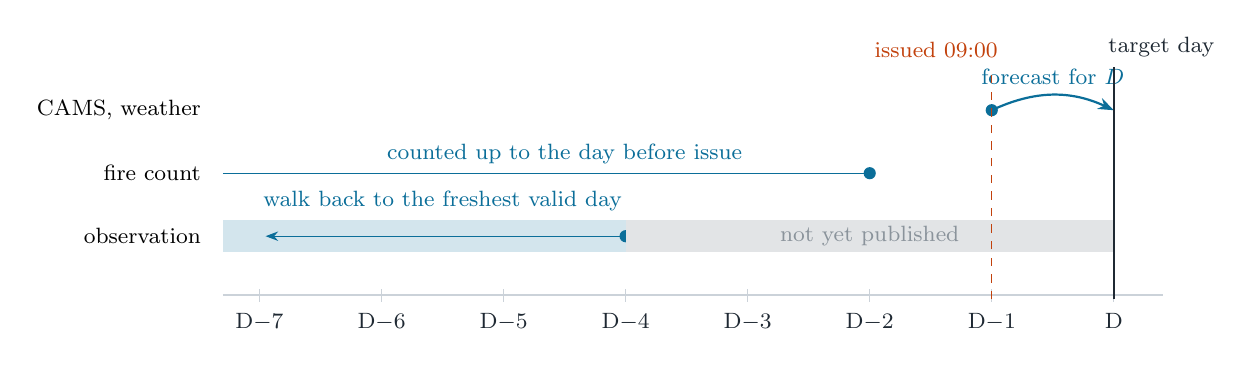
\begin{tikzpicture}[font=\small, x=1.55cm, y=1cm]
  % axis
  \draw[rule, thick] (-0.3,0) -- (7.4,0);
  \foreach \i/\l in {0/D$-$7,1/D$-$6,2/D$-$5,3/D$-$4,4/D$-$3,5/D$-$2,6/D$-$1,7/D}
    { \draw[rule] (\i,-0.08) -- (\i,0.08);
      \node[below, font=\footnotesize, text=ink] at (\i,-0.1) {\l}; }

  % observations
  \fill[accent!18] (-0.3,0.55) rectangle (3,0.95);
  \node[anchor=east, font=\footnotesize] at (-0.4,0.75) {observation};
  \fill[accent] (3,0.75) circle (2.2pt);
  \draw[accent, -{Stealth[length=1.6mm]}] (3,0.75) -- (0.05,0.75);
  \node[above, font=\footnotesize, text=accent] at (1.5,0.95)
    {walk back to the freshest valid day};
  \fill[muted!25] (3,0.55) rectangle (7,0.95);
  \node[font=\footnotesize, text=muted] at (5,0.75) {not yet published};

  % fires
  \node[anchor=east, font=\footnotesize] at (-0.4,1.55) {fire count};
  \fill[accent] (5,1.55) circle (2.2pt);
  \draw[accent] (-0.3,1.55) -- (5,1.55);
  \node[above, font=\footnotesize, text=accent] at (2.5,1.55)
    {counted up to the day before issue};

  % forecasts
  \node[anchor=east, font=\footnotesize] at (-0.4,2.35) {CAMS, weather};
  \draw[accent, thick, -{Stealth[length=2mm]}] (6,2.35) to[bend left=25]
    node[above, font=\footnotesize] {forecast for $D$} (7,2.35);
  \fill[accent] (6,2.35) circle (2.2pt);

  % issue time and target
  \draw[warn, dashed] (6,-0.05) -- (6,2.9) node[above left=0mm and -2mm,
    font=\footnotesize, text=warn] {issued 09:00};
  \draw[ink, thick] (7,-0.05) -- (7,2.9) node[above right=0mm and -2mm,
    font=\footnotesize] {target day};
\end{tikzpicture}
\caption{What the forecast for day $D$ may use. A dot is the newest
value of each input the forecast is allowed to see. Observations
walk back up to three further days when the cutoff day has not
been published or is too thin to count.}
\label{fig:infoset}
\end{figure}

\subsection{Quality rules}

\begin{itemize}
  \item \textbf{Sixteen hours or it does not count.} CPCB treats a
    daily mean built from fewer than 16 hourly readings as invalid,
    and so does Pawan: such days are kept in the table but never
    used as a label or as a later day's persistence. \RowsThin{}
    of \RowsObserved{} observed days fall below the line.
  \item \textbf{Thin days are refreshed.} The feed publishes a day
    as soon as it has some hours and fills the rest in later; the
    ingest replaces a thin reading when more hours arrive.
  \item \textbf{The freshest valid reading, not a fixed day.} The
    feed lands in batches every two to five days. Reading only
    $D-4$ left ten of the first thirty-one target days without a
    forecast; the reader now walks back up to three further days.
\end{itemize}

\subsection{The history, and a mistake worth recording}

Until this iteration the table began on 15 May 2026, because the
first bootstrap requested \texttt{past\_days=92}, on the belief that
92 days was as far back as the CAMS archive went. It is only the
ceiling on that one parameter; an explicit start and end date reach
back to August 2022. The live sensor has reported since February
2025, so the 2025 burning season had been available from the first
day of the project, and the model had been fitted on summer and
monsoon alone.

The consequence was visible in October. On 3 and 5 October the live
forecast was 22~\ugm{} against an observed 38: the model had never
seen the season starting. Extending the table to \RowsFirst{} added
every day of October and November 2025, with no gaps. Refitted on
that history, the backtest forecasts for the same two days are 33
and 42. Rows from archives carry no issue date and are marked as
such; they are training history, never part of the live record.

\section{Method%
  \BvrHint{\ldots deliberately ordinary}}
\label{sec:method}

The model is a ridge regression, refitted from scratch every
morning, predicting $\log(1+y)$ where $y$ is tomorrow's daily mean
\pmtf. Fitting in log space makes the penalty proportional, which
is how the error is felt: ten out on a reading of twenty matters,
ten out on two hundred matters much less. The penalty strength is
chosen inside each fit on the most recent fifth of its own training
window, so it never sees the day being predicted.

\begin{table}[H]
\centering
\small
\begin{tabularx}{\linewidth}{>{\ttfamily}l >{\raggedright\arraybackslash}X r}
\toprule
\normalfont\textbf{Feature} & \textbf{Meaning} & \textbf{Weight} \\
\midrule
cams\_log & log of CAMS's forecast for tomorrow & $+0.197$ \\
obs\_recent\_log & log of the freshest valid observation & $+0.113$ \\
burning & 1 in October and November & $+0.037$ \\
temp, rh & forecast temperature and humidity & $-0.159$, $-0.252$ \\
wind\_speed & forecast wind speed & $-0.124$ \\
wind\_u, wind\_v & wind as eastward and northward components & $+0.042$, $+0.023$ \\
fire\_log & log of the upwind fire count the day before issue & $+0.116$ \\
\bottomrule
\end{tabularx}
\caption{The nine features and their standardised weights in the
model fitted on 10 October. Signs read physically: humid, warm and
windy days are cleaner; fires and a high CAMS forecast push the
estimate up.}
\end{table}

\paragraph{Why not gradient boosting.} The proposal planned a
boosted tree ensemble with a linear model alongside. Two things
changed the plan. Until this iteration there were never more than
about a hundred usable rows, which is too few for trees to beat a
penalised linear fit. And the daily job runs unattended until the
end of the semester, which made a standard-library-only pipeline
worth more than a library dependency. The linear model was
therefore built first, and it is what is reported. With
\Usable{} usable rows now on hand, a boosted model is worth testing
offline, and it is in the plan.

\paragraph{Candidates tested and not adopted.} With a burning season
in the table, four ways of letting the season change the model were
backtested against the current one: season interactions on the fire
count and the eastward wind (smoke transport), on persistence and
CAMS (how far to trust each), all four together, and a separate fit
for burning-season days. The bar was set before the comparison:
clearly better in burning season, no more than a point or two worse
in calm. None cleared it. The best, smoke transport, gained 1.3
points in burning season and lost 1.7 on the live days, which on 63
days is noise. The model was left as it is.

\section{Evaluation%
  \BvrHint{\ldots including the awkward numbers}}
\label{sec:eval}

\subsection{Baselines}
\label{sec:baselines}

\begin{itemize}
  \item \textbf{Operational persistence}: tomorrow equals the
    freshest reading published by 09:00, about four days old. The
    same information Pawan has, so the fair comparison and the bar
    the targets are measured against.
  \item \textbf{Textbook persistence}: tomorrow equals today. The
    baseline the proposal quoted. Nobody has today's reading when
    the forecast goes out, so it marks a ceiling rather than a
    competitor: the gap between the two persistences is the cost of
    the publication lag, and closing it needs a faster feed rather
    than a better model.
  \item \textbf{Raw CAMS}: the uncorrected global forecast.
\end{itemize}

\subsection{Results}

\begin{table}[H]
\centering
\small
\begin{tabular}{l r r r r r r}
\toprule
& \textbf{Days} & \textbf{Pawan} & \textbf{Operational} &
  \textbf{Textbook} & \textbf{Raw CAMS} & \textbf{Skill} \\
\midrule
Calm season & \NCalm & \textbf{\ModelCalm} & \OperCalm & \TextCalm
  & \CamsCalm & $+\SkillOpCalm\%$ \\
Burning season & \NBurn & \textbf{\ModelBurn} & \OperBurn & \TextBurn
  & \CamsBurn & $+\SkillOpBurn\%$ \\
Live rows only & \NLive & \textbf{\ModelLive} & \OperLive & \TextLive
  & \CamsLive & $+\SkillOpLive\%$ \\
\midrule
All & \NAll & \textbf{\ModelAll} & \OperAll & \TextAll & \CamsAll
  & $+\SkillOpAll\%$ \\
\bottomrule
\end{tabular}
\caption{Mean absolute error in \ugm, walk-forward, \BacktestFirst{}
to \BacktestLast. Skill is the reduction against operational
persistence; the targets were 10\% calm and 20\% burning. Live rows
are those whose CAMS forecast was recorded on the day rather than
read back from an archive.}
\label{tab:results}
\end{table}

\begin{figure}[H]
\centering
\begin{tikzpicture}
\begin{axis}[
  width=0.97\linewidth, height=6.2cm,
  xmin=0, xmax=60,
  ymin=0, ymax=150,
  xtick={0,14,31,45,60},
  xticklabels={1 Oct,15 Oct,1 Nov,15 Nov,30 Nov},
  ylabel={daily mean \pmtf, \ugm},
  ylabel style={font=\small},
  tick label style={font=\footnotesize},
  axis lines=left,
  axis line style={rule},
  major tick style={rule},
  ymajorgrids, grid style={rule!50},
  legend style={draw=none, font=\footnotesize, fill=none,
    at={(0.5,1.03)}, anchor=south, legend columns=3,
    /tikz/every even column/.append style={column sep=4mm}},
  legend cell align=left,
]
  \addplot[muted, dashed, thick] table[x=day, y=persistence]
    {data/season.dat};
  \addlegendentry{operational persistence}
  \addplot[ink, thick] table[x=day, y=observed] {data/season.dat};
  \addlegendentry{observed}
  \addplot[accent, very thick] table[x=day, y=model] {data/season.dat};
  \addlegendentry{Pawan, issued the day before}
  \draw[warn, densely dotted] (axis cs:0,90) -- (axis cs:60,90)
    node[pos=0.98, above left, font=\footnotesize, text=warn] {Poor};
\end{axis}
\end{tikzpicture}
\caption{The 2025 burning season, day by day, as the walk-forward
backtest forecast it. Pawan follows the season's level far better
than a four-day-old reading does, and tops out well short of the
peaks.}
\label{fig:season}
\end{figure}

Three things in Table~\ref{tab:results} are worth saying directly.
Both targets are met with room to spare, in the burning season on a
full season of data. The live rows, which no archive has helped,
score better than the backfilled ones, though they cover only the
last two months, so the archive's mild optimism is not what is
carrying the result. And Pawan loses to
textbook persistence in every row, by \LossTxCalm\% in the calm
season and \LossTxBurn\% in the burning one. Most of what the model adds is recovering what the
four-day lag throws away; it is not better than knowing yesterday.

\subsection{What the correction is correcting}

\begin{figure}[H]
\centering
\begin{tikzpicture}
\begin{axis}[
  width=0.97\linewidth, height=5cm,
  ybar, bar width=9pt, bar shift=0pt,
  xmin=0.4, xmax=12.6, ymin=0, ymax=4.4,
  xtick={1,...,12},
  xticklabels={Jan,Feb,Mar,Apr,May,Jun,Jul,Aug,Sep,Oct,Nov,Dec},
  ylabel={CAMS $\div$ observed},
  ylabel style={font=\small},
  tick label style={font=\footnotesize},
  axis lines=left, axis line style={rule}, major tick style={rule},
  ymajorgrids, grid style={rule!50},
]
  \addplot[fill=muted!60, draw=none] table[x=month, y=ratio,
    restrict x to domain=1:9] {data/ratio.dat};
  \addplot[fill=accent, draw=none] table[x=month, y=ratio,
    restrict x to domain=10:11] {data/ratio.dat};
  \addplot[fill=muted!60, draw=none] table[x=month, y=ratio,
    restrict x to domain=12:12] {data/ratio.dat};
  \draw[ink, densely dashed] (axis cs:0.4,1) -- (axis cs:12.6,1)
    node[pos=0.01, above right, font=\footnotesize, fill=white,
    inner sep=1pt] {unbiased};
\end{axis}
\end{tikzpicture}
\caption{How far CAMS overshoots, by month, February 2025 to October
2026. It reads \RatioHigh{} times the observed value in the monsoon
and \RatioLow{} times in November (burning months in blue). A single
scale factor cannot correct both, which is why the correction
depends on weather and season.}
\label{fig:ratio}
\end{figure}

\subsection{What it gets wrong}
\label{sec:fails}

\begin{itemize}
  \item \textbf{It does not see spikes.} Of the \PoorDays{} days
    that reached the \emph{Poor} band, Pawan flagged none; its
    highest forecast anywhere in the backtest is \MaxForecast~\ugm.
    On the five worst days it forecast, on average, \TopFiveRatio\%
    of what was observed; on \PeakDay{} the station read \PeakObs{}
    and the forecast was \PeakModel. One band lower, of \ModDays{}
    days worse than \emph{Satisfactory} it caught \ModCaught{},
    against \ModOperCaught{} for operational persistence. Part of
    the gain in average error comes from forecasting towards the
    middle, which is the right trade for an ordinary day and the
    wrong one for an advisory.
  \item \textbf{The likely range is too narrow.} The published band
    is meant to hold about four days in five. On the \LiveScored{}
    scored live forecasts it held \LiveInside.
  \item \textbf{The live service missed days.} Between \LiveFirst{}
    and \LiveLast{} it issued \LiveIssued{} of \LiveExpected{}
    forecasts. Most of the misses came from the fixed-day observation
    rule; the fix was merged on 10 October.
  \item \textbf{Backfilled rows are mildly optimistic.} Archive CAMS
    and weather are stitched from the opening hours of successive
    model runs. The live-only row in Table~\ref{tab:results} is the
    check on this, and so far it agrees.
\end{itemize}

\section{Engineering log%
  \BvrHint{\ldots found, fixed, guarded}}
\label{sec:log}

Every fault below was found in the running system, fixed through a
pull request, and left behind a test or a run-time check so that it
cannot come back quietly. The weekly journals tell each one in full.

\begin{table}[H]
\centering
\small
\begin{tabularx}{\linewidth}{l >{\raggedright\arraybackslash}X >{\raggedright\arraybackslash}X}
\toprule
\textbf{Week} & \textbf{What went wrong} & \textbf{Guard left behind} \\
\midrule
2 & The observation API ignored misspelt date filters and returned
  the whole series, which made a sensor dead since 2022 look like
  the better one. & Dates re-checked client side; the live sensor id
  pinned in config with the reason. \\
3 & The persistence baseline in the proposal used a reading that
  does not exist at issue time. & Two persistences reported side by
  side; a test that features never see past the publication lag. \\
4 & The ingest called the wrong endpoint and committed nothing new
  for three weeks while reporting success. & Staleness tripwire:
  the run fails if the freshest reading is over seven days old. \\
5 & The model lost to persistence by 22.6\%, from leaked fire
  counts, a seasonal term acting as a trend, and thin days used as
  labels. & Fire count lagged; sixteen-hour rule; tests for each. \\
Oct & Ten of thirty-one target days had no forecast; the page showed
  a stale one as tomorrow's; a clock-dependent test would have
  blocked data commits from 22 October. & Walk-back reader; status
  block and honest empty card; test dates pinned. \\
Oct & The history began in May because a request parameter limit
  was mistaken for the archive's. & Extension script and a dry-run
  workflow; \texttt{bootstrap.py} refuses to overwrite the table. \\
\bottomrule
\end{tabularx}
\caption{Faults found in operation.}
\end{table}

\section{Improvement plan%
  \BvrHint{\ldots week 8 onwards}}
\label{sec:plan}

In priority order. Each item has a test that says whether it
worked, decided before it is tried.

\begin{enumerate}[leftmargin=0.7cm]
  \item \textbf{See the spikes.} Add an exceedance forecast
    alongside the point forecast, the probability that tomorrow is
    worse than \emph{Satisfactory}, and correct the log-space
    back-transform, which currently returns something closer to a
    median than a mean. \emph{Done when} recall on days above
    60~\ugm{} beats operational persistence's \ModOperCaught{} of
    \ModDays{} without more false alarms than it.
  \item \textbf{Calibrate the likely range} from the backtest's own
    residuals by season, instead of one spread for the year.
    \emph{Done when} the band holds between 75 and 85\% of days.
  \item \textbf{Score the 2026 season live.} October and November
    are the test nothing here was tuned against. The results page
    already separates live rows; the final report will lead with
    them.
  \item \textbf{A second burning season in April and May.} The fire
    box sees more detections during wheat residue burning than in
    November, but the \texttt{burning} flag covers only October and
    November. Test a flag for both, by the same pre-set bar as the
    candidates above.
  \item \textbf{Try boosted trees offline}, now that there are
    \Usable{} usable rows, with the linear model as the reference.
    Adopted only if it wins on both seasons and the live rows.
  \item \textbf{An interactive layer} on the project page, if time
    allows after the above.
\end{enumerate}

\section{Risks}

\begin{itemize}
  \item \textbf{One season is one season.} The burning-season result
    rests on 2025 and the first days of 2026. A wetter or drier
    year, or a shift in when the stubble is burnt, would move it.
  \item \textbf{The feed lag sets a ceiling.} Pawan cannot beat a
    reading it does not have. A faster observation source would do
    more for accuracy than any model change.
  \item \textbf{Upstream change.} CAMS is upgraded from time to time
    and its bias could shift between seasons. The live-only score is
    the early warning.
  \item \textbf{Platform drift.} GitHub moves its default runner to
    a new Ubuntu release on 19 October. The workflows are pinned to
    the current one so the daily job does not change underneath the
    project before the final seminar.
\end{itemize}

\section{Reproducing this report}

Every number above is generated from the repository's data. From a
fresh clone:

\begin{center}
\begin{minipage}{0.8\linewidth}
\small
\begin{verbatim}
pip install -r requirements.txt
python code/evaluate.py
python scripts/report_figures.py
cd project-report-prototype-stage
latexmk -pdf main.tex
\end{verbatim}
\end{minipage}
\end{center}

The figures here are a snapshot of the record on 10 October 2026.
The results page on the project site is regenerated every morning
and is the current one.

\end{document}
